%% ================================================
%% SPECULATIVE / WIP — Not part of CORE claims.
%% ================================================
\section{Appendix J: Visual Maps of UBT 2.0}
\label{app:visual-maps}

This appendix collects navigational diagrams for UBT 2.0. Each figure is a high-level map with cross-references to the main text and appendices.

\subsection{Global structure}
\begin{figure}[h]
  \centering
  %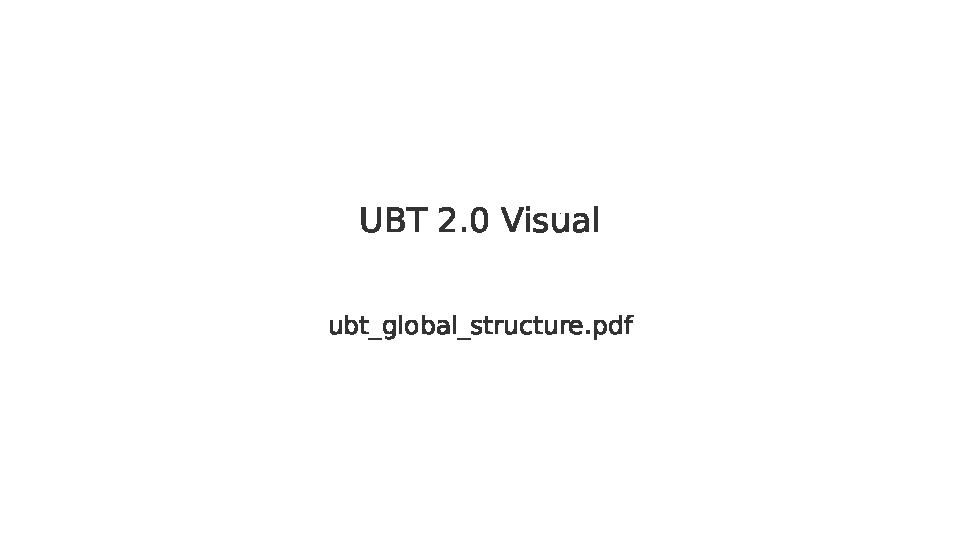
\includegraphics[width=\textwidth]{img/ubt_global_structure.pdf}
  \caption{Global UBT map: Gravity (A), Scalar/Imaginary (B), EM (C), QED/Dirac (D), SM+QCD (E), Psychons/Resonator (F,T), Dark Matter (G), Alpha+p-adic (H), New Fields (I), Visual Maps (J), Fundamental Constants (K), Dark Energy (M), p-adic overview (O), Bibliography (P).}
  \label{fig:ubt-global-map}
\end{figure}

\subsection{Alpha and p-adic pipeline}
\begin{figure}[h]
  \centering
  %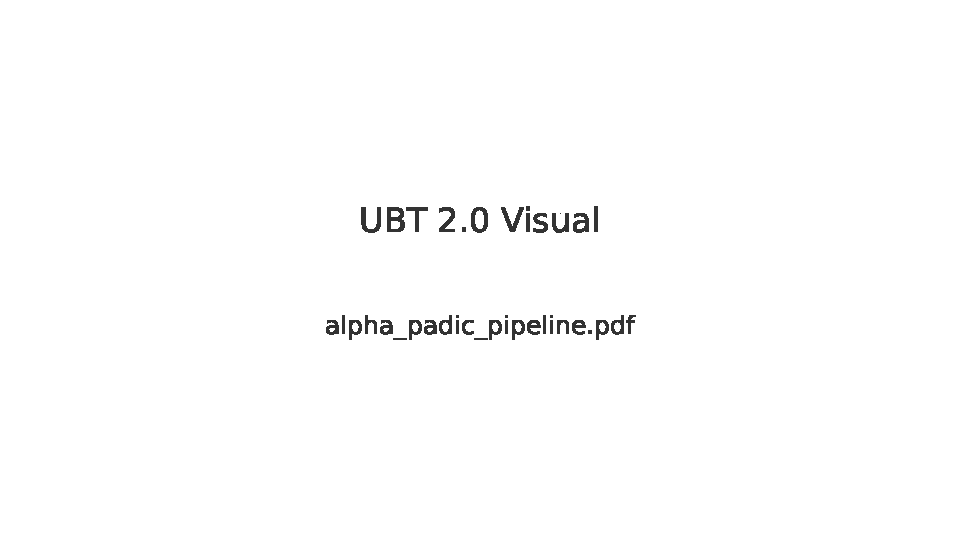
\includegraphics[width=\textwidth]{img/alpha_padic_pipeline.pdf}
  \caption{Pipeline from topological integer $N$ to the renormalized $\alpha$ (Appendix~\ref{app:alpha-consolidated}), and p-adic branches (Appendix~\ref{app:padic-rigorous}, \ref{app:dm-consolidated}).}
  \label{fig:alpha-padic-pipeline}
\end{figure}

\subsection{Dark matter sector maps}
\begin{figure}[h]
  \centering
  %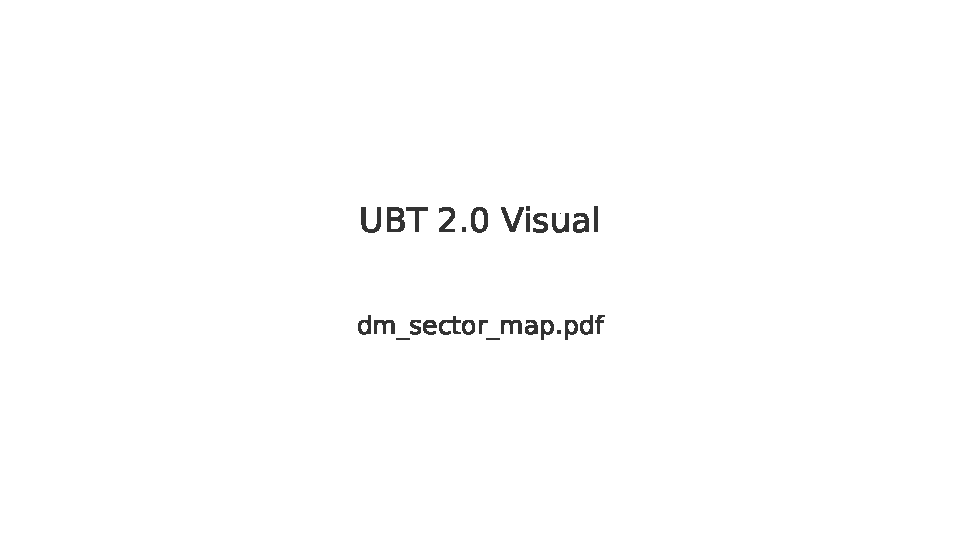
\includegraphics[width=\textwidth]{img/dm_sector_map.pdf}
  \caption{Dark matter sector pathways: Hopfions and knotted modes (Appendix~\ref{app:dm-consolidated}) and prime/$p$-adic hidden sectors.}
  \label{fig:dm-sector-map}
\end{figure}

\subsection{Experimental interfaces}
\begin{figure}[h]
  \centering
  %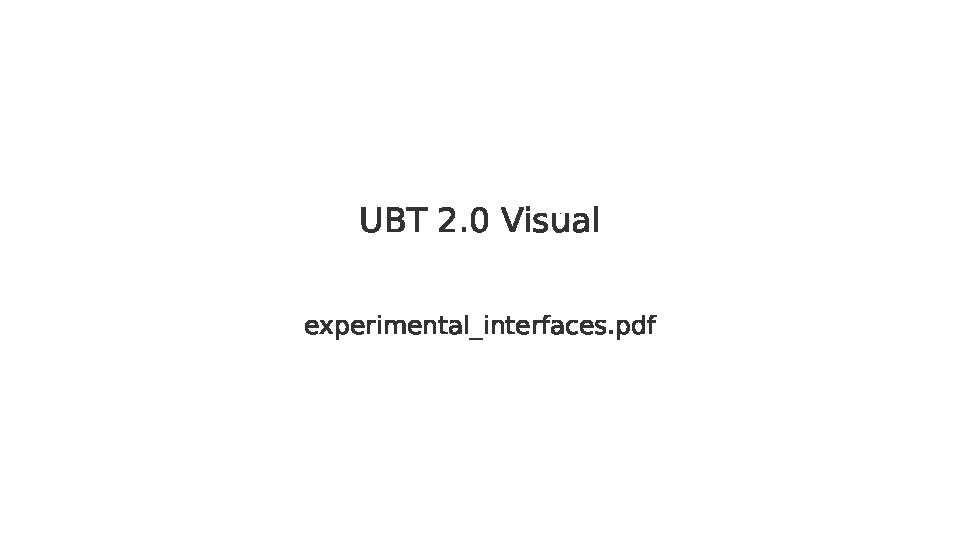
\includegraphics[width=\textwidth]{img/experimental_interfaces.pdf}
  \caption{Experimental interfaces: Theta resonator (Appendix~T), EM in curved space (Appendix~K), SM/QCD portals (Appendix~\ref{app:sm-qcd-ubt}).}
  \label{fig:experimental-interfaces}
\end{figure}
